\documentclass[12pt]{article} 
\usepackage[left=20mm, top=16mm, right=16mm, bottom=20mm]{geometry} 
\usepackage{graphicx}
\usepackage{wrapfig}
\graphicspath{{../pictures/}}
\DeclareGraphicsExtensions{.pdf,.png,.jpg,.eps}
\usepackage{cmap}					% поиск в PDF
\usepackage{mathtext} 				% русские буквы в формулах
\usepackage[T2A]{fontenc}	
\usepackage[utf8x]{inputenc} 
\usepackage[russian]{babel} 
\usepackage{amsmath,amsfonts,amssymb,amsthm,mathtools} 
\usepackage{icomma} % "Умная" запятая: $0,2$ --- число, $0, 2$ --- перечисление
\usepackage{euscript}	 % Шрифт Евклид
\usepackage{mathrsfs} % Красивый матшрифт
\usepackage{indentfirst}     % Отступ в первом абзаце
%% Перенос знаков в формулах (по Львовскому)
\newcommand*{\hm}[1]{#1\nobreak\discretionary{}
	{\hbox{$\mathsurround=0pt #1$}}{}}

%% Свои команды
%DeclareMathOperator{\sgn}{\mathop{sgn}}
\newcommand{\te}{\ensuremath{\Rightarrow}}
\newcommand{\y}{\ensuremath{\angle}}
\newcommand{\ABC}{\ensuremath{\triangle ABC\,}}
\newcommand{\tr}{\ensuremath{\triangle}}
\newcommand{\ca}{\ensuremath{\cos\alpha}}
\newcommand{\sa}{\ensuremath{\sin\alpha}}
\newcommand{\cb}{\ensuremath{\cos\beta}}
\newcommand{\sib}{\ensuremath{\sin\beta}}
\newcommand{\x}{\cdot}
%DeclareMathOperator{\Sum}{\mathop{Sum}}
\DeclareMathOperator{\Sum}{\mathop{Sum}}

\begin{document}
%DeclareMathOperator{\Sum}{\mathop{Sum}}
\begin{titlepage}		
\begin{center}
\large 	Московский физико-технический университет \\
Факультет общей и прикладной физики \\
\vspace{0.2cm}
Учебная программа\\
"<Квантовая теория поля, теория струн и математическая физика">

\vspace{4.5cm}
II семестр 2016-2017 учебного года \\
\large Домашнее задание №1: \\ \vspace{0.1cm}
\LARGE \textbf{Правильные многогранники}
\end{center}
\vspace{2.3cm} \large

\begin{center}
		 Автор: \\
 Иванов Кирилл,
 625 группа
\vspace{10mm}


\end{center}

\begin{center} \vspace{50mm}
г. Долгопрудный \\ 
4 марта 2017 года
\end{center}
\end{titlepage}


\section{Задание №1}

\textbf{Правильный многогранник }— это выпуклый многогранник, состоящий из одинаковых правильных многоугольников и обладающий пространственной симметрией.  \par 

Необходимые свойства правильного многогранника: 
\begin{enumerate}

\item Он выпуклый;
\item Все его грани являются равными правильными многоугольниками;
\item В каждой его вершине сходится одинаковое число рёбер.

\end{enumerate}

Всего существует 5 правильных многогранников, перечислим их: \textbf{тетраэдр, октаэдр, гексаэдр, икосаэдр, додекаэдр}. Пусть $ V, E, F $ -- число вершин, рёбер и граней соответственно, тогда для них выполняется теорема Эйлера: 
 \begin{equation}
V - E + F = 2
 \end{equation}
Обозначив за $m,n$  число рёбер, сходящихся в каждой вершине и  число рёбер в каждой грани соответственно, мы получаем важное следствие: 

\begin{equation}
\left\{
\begin{aligned}
&mV= 2E  \\
&nF = 2E\\
\end{aligned}
\right.
\te \dfrac{2}{m} + \dfrac{2}{n} = 1 + \dfrac{2}{E} > 1
\end{equation}

Из (2) понятно, что при больших значениях $m, n$ условие последнего уравнения не будет выполнятся, т.е. существует конечное число наборов $m, n \te $ существует конечное число правильных многогранников. При этом понятно, что $m, n \geqslant 3$.  Простым перебором получаем, что наши искомые 5 многогранников существуют при $ m, n  \in [3;5]$. 

\section{Задание №2}
\begin{wrapfigure}{r}{0.32\linewidth} 
	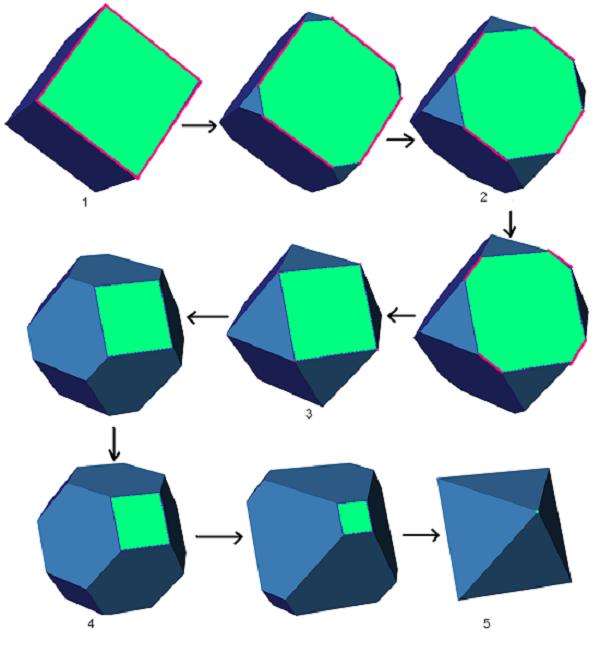
\includegraphics{1_2}
	\caption{Пример перехода от куба к октаэдру}
\end{wrapfigure}
\textbf{Многогранник, дуальный к заданному многограннику} — многогранник, у которого каждой грани исходного многогранника соответствует вершина дуального, каждой вершине исходного — грань дуального и каждому ребру исходного~--~ребро дуального. Многогранник, дуальный дуальному, гомотетичен исходному. 

\textbf{Самодуальные многогранники}— это те многогранники, дуальные которым имеют в точности ту же связь между вершинами, рёбрами и гранями.

Пары правильных дуальных многогранников:
\begin{enumerate}
	\item Тетраэдр -- Тетраэдр
	\item Куб -- Октаэдр
	\item Икосаэдр -- Додекаэдр
\end{enumerate}

\newpage
\section{Задание №3}
Пусть у нас есть пространство $ E $, на котором задано множество $ M $. Тогда \textbf{группа симметрий} этого множества -- множество движений пространства $ E $, переводящих наше множество $ M $ само в себя, т.е.:
\begin{equation}
\Sum M = \{ f \in \Sum E \; | f(M) = M\}
\end{equation}
Таким образом, для правильных многогранников группа симметрий -- множество таких преобразований, переводящие их в самих себя. Такие множества являются математическими группами.

\section{Задание №4}
\textbf{Симметрии куба} делятся на два типа — самосовмещения, при которых точки куба не изменяют своего положения относительно друг друга, и преобразования, оставляющие куб в целом на месте, но передвигающие его точки относительно друг друга. Преобразования первого типа будем называть вращениями. Все вращения образуют группу, которая называется группой
вращений куба.

Имеется ровно 24 вращения куба вокруг различных осей симметрий. В самом деле, при поворотах куба место нижней грани может занять
любая из 6 граней куба (рис. 2). Для каждой из 6 возможностей — когда указано, какая именно грань расположена внизу, — имеется 4 различных расположения куба, соответствующих его поворотам вокруг оси, проходящей через центры верхней и нижней граней, на углы $ 0, \pi/2, \pi, З\pi/2 $. Таким образом, получаем 6×4 = 24 вращений куба. 

Кроме того, куб имеет три плоскости симметрии, проходящие через его центр. Симметрии относительно этих плоскостей в сочетании со всеми вращениями куба дают нам еще 24 преобразования, являющихся самосовмещениями куба. \textbf{Поэтому полная группа симметрий куба состоит из 48 преобразований.}

\begin{wrapfigure}{l}{0.25\linewidth} 
	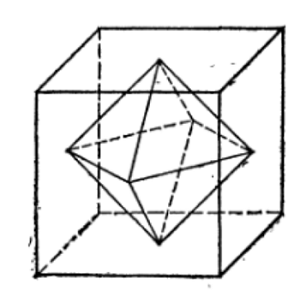
\includegraphics{1_4}
	\caption{Связь куба и октаэдра}
\end{wrapfigure}
Октаэдр один из пяти правильных
многогранников. Его можно получить, соединяя центры граней куба и рассматривая тело, ограниченное плоскостями, которые определяются соединительными прямыми для соседних граней (рис. 3). Поэтому любая симметрия куба одновременно является симметрией октаэдра и наоборот. Таким образом, \textbf{группа симметрий октаэдра такая же, как и группа симметрий куба, и состоит из 48 преобразований.}

\section{Задание №5}

Обозначив за $ \ell $ число плоских углов многогранника, в общем виде можно доказать следующее утверждение: 
\begin{equation}
|\Sum M| = 2\ell
\end{equation}
Это утверждение несложно проверить на группе симметрий тетраэдра ($|\Sum M| = 24)$ и на уже найденных нами группах куба и октаэдра. 

Тогда, учитывая, что у икосаэдра 20 граней с тремя углами, а у додекаэдра -- 12 граней с 5 углами, мы получаем, что \textbf{их группа симметрий состоит из 120 преобразований.}



%%%%%%%%%%%%%%%%%%%%%%%%%%%%%%%
%%%%%%%%%%%%%%%%%%%%%%%%%%%%%%%
\end{document}
